\documentclass[]{article}
\usepackage[T2A]{fontenc}
\usepackage[utf8]{inputenc}
\usepackage[russian]{babel}
\usepackage{amsmath}
\usepackage{amsmath, amsfonts, amssymb, amsthm, mathtools}
\usepackage[left=20mm, top=15mm, right=15mm, bottom=20mm, nohead, nofoot]{geometry}
\usepackage{graphicx}
\usepackage{float}%"Плавающие" картинки
\usepackage{wrapfig}%Обтекание фигур (таблиц, картинок и прочего)
\usepackage{listings}
%opening
\begin{document}
	\begin{titlepage}
		\begin{center}
			\large Санкт-Петербургский политехнический университет Петра Великого \\
			\large Физико-механический институт \\
			\large Высшая школа теоретической механики и математической физики \\[2cm] % [] - отступ
			\large Направление подготовки \\
			\large 01.03.03 Механика и математическое моделирование \\[2cm]
			\LARGE \textbf {Отчёт по лабораторной работе №2} \\[0.5cm]
			\LARGE \textbf {Тема: "Уравнение колебания струны"} \\[0.5cm]
			\large Дисциплина "Вычислительная механика" \\[4cm]
		\end{center}
			\begin{minipage}{0.25\textwidth} % врезка в половину ширины текста
				\begin{flushright}
				\large\textbf{Выполнил:}\\
				\large Работинский А.Д. \\
				\large {Группа:} 5030103/10001 \\
				\large \textbf{Преподаватель:}\\
				\large Е.Ю. Витохин
			\end{flushright}
		\end{minipage}
	\mbox{}
	\vfill
\begin{center}
	\large Санкт-Петербург \\
	\large 2022 
\end{center} 
	\end{titlepage}
	
	\newpage
	\section*{1) Постановка задачи}
		Решается уравнение колебаний струны:
		$\frac{\partial^2{\text{u}}}{\partial{\text{x}^2}}-\frac{1}{\text{c}^2}\frac{\partial^2{\text{u}}}{\partial{\text{t}^2}}=0$ \\
		, где коэффициент $\text{c}=1$\\
		Граничные условия: $\text{u}(0,t)=\phi_0(t) \quad \text{u}(l,t)=\phi_l(t)$\\
		Начальные условия:$\text{u}(x,0)=\psi_0(x) \quad \dot{u}(x,0)=\psi^*(x)$\\
		Конечно-разностные схемы строятся схожим образом, но при решении данной задачи стоит помнить, что должно быть выполнено условие Куранта, иначе в силу отсутствия  устойчивости, явная схема даст неверное решение: \begin{center}
			$\Delta\text{t}<<\frac{h}{c}$
		\end{center}
		$\quad$ В нашем случае граничные условия имеют следующий вид:\\
		\mbox{$\dot{u}(x,0)=x^2(x+1) \quad u(x,0)=x^2cos(\pi x) \quad u(l,t)=t-1 \quad u(0,t)=\phi_0(t)$}
		Шаг по пространству: $h=0.1 $ , шаг по времени \mbox{$\Delta t =0.01$} 
		
	\section*{2)Явная схема интегрирования}
		Конечно-разностные апроксимации получаются схожим образом - из разложения в ряд Тейлора:\\
		\[u(x_0 + h) = u(x_0) + \frac{h}{1!} u^\prime (x_0) + \frac{h^2}{2!}   u^{\prime \prime} (x_0) + o(h^2)\]
		\[
		u(x_0 - h) = u(x_0) - \frac{h}{1!} u^\prime (x_0) + \frac{h^2}{2!} u^{\prime \prime} (x_0) + o(h^2)
		\]
		\begin{center}
			Осталось разрешить систему относительно $u^{\prime \prime} (x_0)$:
		\end{center}
		\[
		u^{\prime \prime} (x_0) = \frac{u(x_0 + h) - 2u(x_0) + u(x_0 -h)}{h^2}
		\]
		\begin{center}
		Разложим в ряд Тейлора функцию перемещений около точки $t_0$:
		\end{center}
		\[
		u(t_0 + \Delta t) = u(t_0) + \frac{\Delta t}{1!} \dot{u} (t_0) + \frac{\Delta t^2}{2!} \ddot{u} (t_0) + o(\Delta t^2)
		\]
		\[
		u(t_0 - \Delta t) = u(t_0) - \frac{\Delta t}{1!} \dot{u} (t_0) + \frac{\Delta t^2}{2!} \ddot{u} (t_0) + o(\Delta t^2)
		\]
		\begin{center}
		Получаем апроксимацию для: $\ddot{u} (t_0)$:\\
		\end{center}
		\[
		\ddot{u} (t_0) = \frac{u(t_0 + \Delta t) - 2u(t_0) + u(t_0 - \Delta t)}{\Delta t^2}
		\]\\
		Введем сетку следующим образом:
		\begin{center}
			$x=ih \quad x \in \text{[0;N]}$ 
 			\[t=kh \quad k \in \text{[0;K]}\]			
		\end{center}
		Итого получаем выражение для интегрирования по явной схеме:\\
		\begin{center}
			\fbox{$\text{u}_i^{k+1}=\frac{c^2\Delta t^2}{h^2}(\text{u}_{i+1}^k-2\text{u}_i^k+\text{u}_{i-1}^k)+2\text{u}_i^k-\text{u}_i^{k-1}$}
		\end{center}
		\subsection*{Получившиеся результаты:}
		\begin{figure}[H]
			\centering
			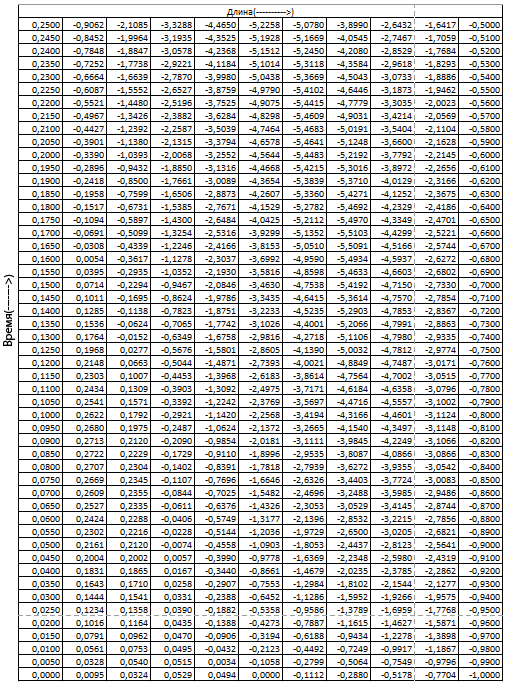
\includegraphics[width=0.8\textwidth]{tab1}
			\caption{Таблица перемещений явной схемы}
			\label{pиc1}
		\end{figure}
		\begin{figure}[H]
			\centering
			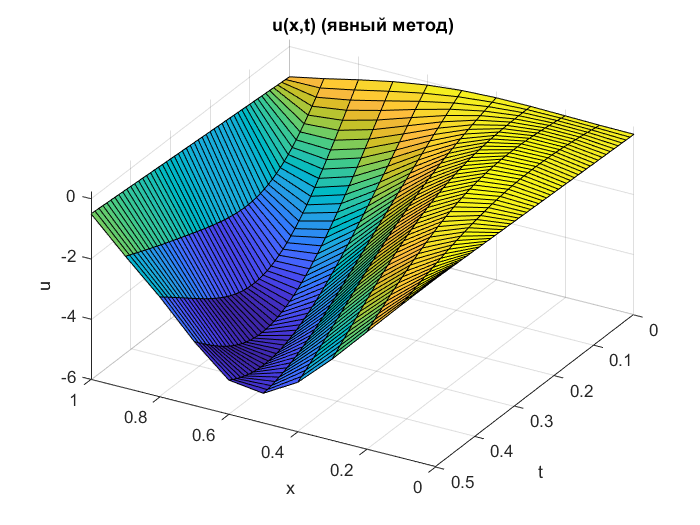
\includegraphics[width=\textwidth]{surfyavn}
			\caption{График u(x,t)}
			\label{pиc2}
		\end{figure}
	\section*{2)Неявный метод}
		Используя выражения производных по координате и времени от u выше и уравнение колебаний $\frac{\partial^2 u}{\partial t^2} = \frac{\partial^2 u}{\partial x^2}$, получим СЛАУ, которую приводим к более общему виду:\\
		\begin{center}
			\fbox{$-Au_{i-1}^{k+1} + Bu_i^{k+1} - Cu_{i+1}^{k+1} = F_i$}
		\end{center}
		,где $A = \frac{1}{h^2}, B = \frac{2\Delta t^2 c^2+h^2}{\Delta t^2 h^2}, C =  \frac{1}{h^2}, F_i = \frac{2}{\Delta t^2}u_i^k - \frac{1}{\Delta t^2}u_i^{k-1}$.\\
		Это уравнение представляет из себя СЛАУ, причем матрица этой системы трехдиагональна, таким образом ее целесообразно решать методом прогонки:\\
		\[\begin{pmatrix}
			1&0&0&0&0&\dots&0\\
			-A&B&-C&0&\dots&\dots&0\\
			0&-A&B&-C&\dots&\dots&0\\
			\dots&\dots&\dots&\dots&\dots&\dots&\dots\\
			0&0&\dots&\dots&-A&B&-C\\
			\dots&\dots&\dots&\dots&\dots&\dots&1
		\end{pmatrix}
		\begin{pmatrix}
			u_0^{k+1}\\
			u_0^{k+1}\\
			u_0^{k+1}\\
			\vdots\\
			u_{N-1}^{k+1}\\
			u_{N}^{k+1}\\
		\end{pmatrix}
	=
	\begin{pmatrix}
		u_0^{k+1}\\
		F_0^{k+1}\\
		F_0^{k+1}\\
		\vdots\\
		F_{N-1}^{k+1}\\
		u_{N}^{k+1}\\
	\end{pmatrix}
	\]
	\newpage
	Для того, чтобы сохранить второй порядок точности необходимо,чтобы было выполнено следующее условие:\\
	\begin{center}
	\fbox{$u_i^1=\psi_0(x)+\psi^*(x)\Delta t + \frac{(\Delta t)^2c^2}{2h^2}(\psi_{0,i-1}-2\psi_{0,i}+\psi_{0,i+1})$}
	\end{center}
	\subsection*{Получившиеся результаты:}
			\begin{figure}[H]
			\centering
			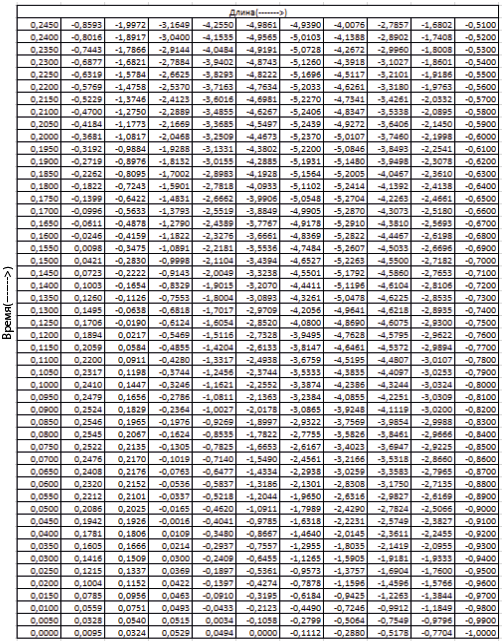
\includegraphics[width=0.8\textwidth]{tab2}
			\caption{Таблица перемещений неявной схемы}
			\label{pиc3}
		\end{figure}
	\newpage
	\subsection*{Получившиеся результаты:}
	\begin{figure}[H]
		\centering
		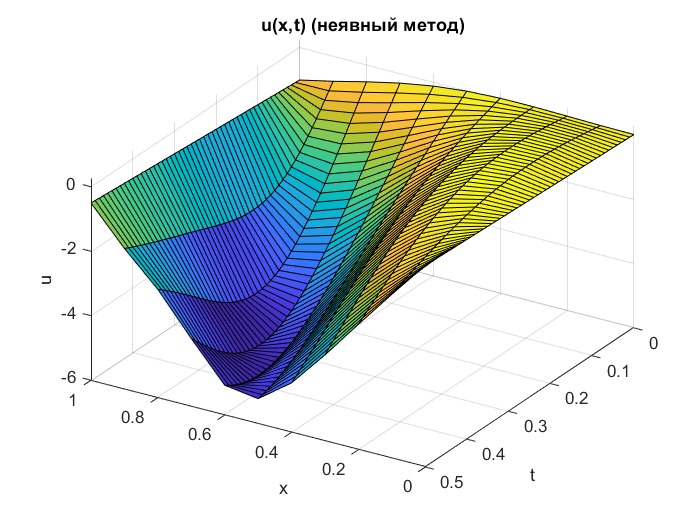
\includegraphics[width=0.8\textwidth]{surfnotyavn}
		\caption{График u(x,t)}
		\label{pиc4}
	\end{figure}
	\newpage
	\section*{Сравнение результатов:}
	Из графиков ниже,заметим, что методы дают очень близкие результаты, что говорит о правильности решения задачи.\\
	\begin{figure}[H]
		\centering
		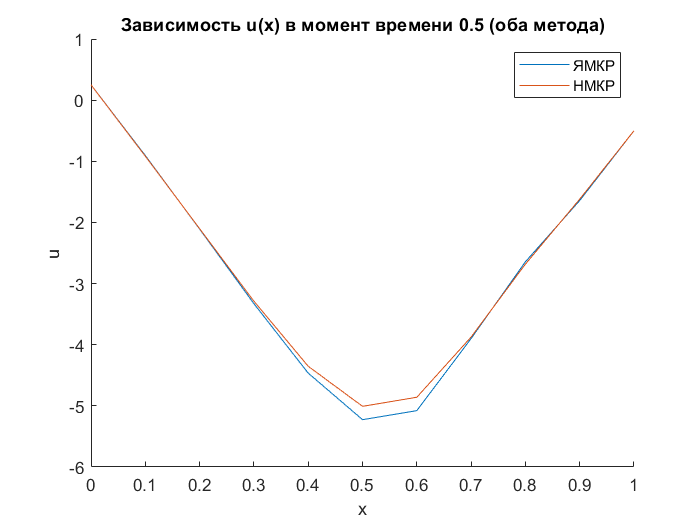
\includegraphics[width=0.7\textwidth]{zav05}
		\caption{График u(x,t) в момент времени 0.5}
		\label{pиc5}
	\end{figure}
	\begin{figure}[H]
		\centering
		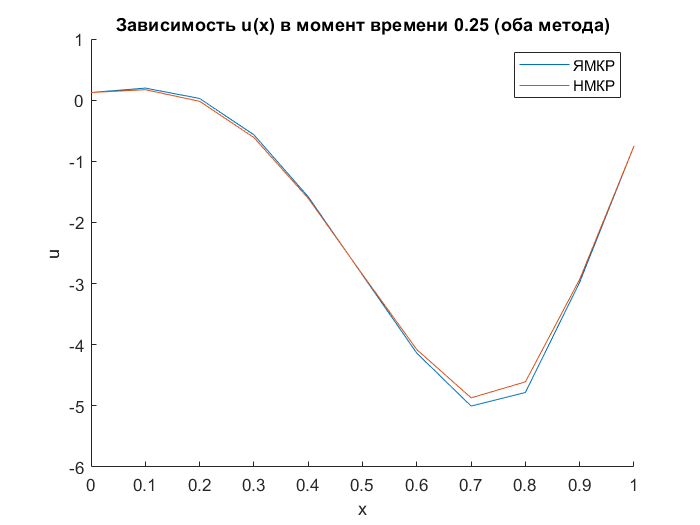
\includegraphics[width=0.7\textwidth]{zav025}
		\caption{График u(x,t) в момент времени 0.25}
		\label{pиc6}
	\end{figure}
	\begin{figure}[H]
		\centering
		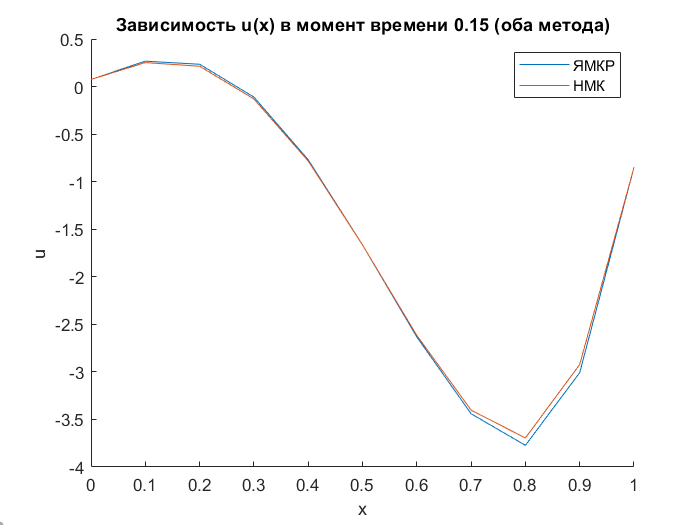
\includegraphics[width=0.7\textwidth]{zav015}
		\caption{График u(x,t) в момент времени 0.15}
		\label{pиc7}
	\end{figure}
\newpage
	\section*{Код (выполнен в MATLAB)}
	\begin{lstlisting}
		t=[0:0.01:0.5];
		x=[0:0.1:1];
		dt=0.01;
		h=0.1;
		n=(1/0.1)+1;
		k=0.5/0.01+1;
		u=zeros(k,n);
		u1=zeros(k,n);
		u_dop=zeros(n,1);
	\end{lstlisting}
	Заполняю ГУ\\
	\begin{lstlisting}
		for i=1:n
		u(k,i)=((i-1)*h)^2*cos(pi*(i-1)*h);
		u1(k,i)=((i-1)*h)^2*cos(pi*(i-1)*h);
		%    u(k,i)=2*((i-1)*h)*((i-1)*h+1)+0.3;
		%    u1(k,i)=2*((i-1)*h)*((i-1)*h+1)+0.3;
		end
		for i=k:-1:1
		u(i,1)=0.5*((k-i)*dt);
		u1(i,1)=0.5*((k-i)*dt);
		%    u(i,1)=0.3;
		%    u1(i,1)=0.3;
		end
		for i=k:-1:1
		u(i,n)=(k-i)*dt-1;
		u1(i,n)=(k-i)*dt-1;
		%    u(i,n)=4.3+(i-1)*dt;
		%    u1(i,n)=4.3+(i-1)*dt;
		end
		\end{lstlisting}
		 Первая строка перемещений\\
		\begin{lstlisting}
		for i=2:n-1
		u1(k-1,i)=((i*h)^2*cos(pi*i*h))+((i*h)^2*(i*h+1))*dt+....
		+(dt^2/(2*h^2))*((((i-1)*h)^2*cos(pi*(i-1)*h))-2*(((i)*h)^2*cos(pi*i*h))...
		+(((i+1)*h)^2*cos(pi*(i+1)*h)));
		u(k-1,i)=((i*h)^2*cos(pi*i*h))+((i*h)^2*(i*h+1))*dt+...
		+(dt^2/(2*h^2))*((((i-1)*h)^2*cos(pi*(i-1)*h))-2*(((i)*h)^2*cos(pi*i*h))+...
		+(((i+1)*h)^2*cos(pi*(i+1)*h)));
		%    ((i-1)*h)^2*cos(pi*(i-1)*h)+(((i-1)*h)^2*((i-1)*h+1))*dt+...
		+(dt^2/(2*h^2))*(((i-1)*h)^2*cos(pi*(i-1)*h)-2*((i)*h)^2*cos(pi*(i)*h)+...
		+((i+1)*h)^2*cos(pi*(i+1)*h));
		end
	\end{lstlisting}
		 Решение задачи по явному мкр\\
	\begin{lstlisting}
		for j=k-1:-1:2
		for i=2:n-1
		u(j-1,i)=(dt^2/(h^2))*(u(j,i+1)-2*u(j,i)+u(j,i-1))+2*u(j,i)-u(j+1,i);
		end
		end
	\end{lstlisting}
	Решение задачи по неявному мкр\\
	\begin{lstlisting}
		A=-1/(h^2);
		B=(h^2+2*dt^2)/((dt^2)*(h^2));
		C=-1/(h^2);
	\end{lstlisting}
	 Заполняю матрицу коэффициентов\\
	 \begin{lstlisting}
		matrix=zeros(n);
		for i=2:n-1
		matrix(i,i)=B;
		matrix(i,i-1)=-A;
		matrix(i,i+1)=-C;
		end
		matrix(1,1)=1;
		matrix(n,n)=1;
		
		
		for j=k-1:-1:2
		del=zeros(n,1);
		lam=zeros(n,1);
		F=zeros(n,1);
		
		P(1)=-C/B;
	\end{lstlisting}
		 Реализуем сам метод прогонки\\
		 прямой ход\\
	\begin{lstlisting}
		for i=1:n
		F(i)=(2*u1(j,i))/(dt^2)-u1(j+1,i)/(dt^2); 
		end
		Q(1)=F(1)/B;
		for i=2:n
		P(i)=-C/(B+A*P(i-1));
		Q(i)=(F(i)-A*Q(i-1))/(B+A*P(i-1));
		end
	\end{lstlisting}
	Обратный ход
	\begin{lstlisting}
		for i=n-1:-1:2
		u1(j-1,i)=P(i)*u1(j-1,i+1)+Q(i); 
		end
		end
		temp=zeros(1,n);
		temp1=zeros(1,n);
		for i=1:(k-1)/2
		temp=u(i,:);
		u(i,:)=u(k-i+1,:);
		u(k-i+1,:)=temp;
		temp1=u1(i,:);
		u1(i,:)=u1(k-i+1,:);
		u1(k-i+1,:)=temp1;
		end
		figure()
		hold on
		grid on
		surf(x,t,u);
		xlabel('x')
		ylabel('t')
		zlabel('u')
		figure()
		surf(x,t,u1);
		xlabel('x')
		ylabel('t')
		zlabel('u')
		figure()
		hold on
		plot(x,u(16,:));
		plot(x,u1(16,:));
		xlabel('x')
		ylabel('u')
		figure()
		hold on
		plot(x,u(k,:));
		plot(x,u1(k,:));
		xlabel('x')
		ylabel('u')
		figure()
		hold on
		plot(x,u(26,:));
		plot(x,u1(26,:));
		xlabel('x')
		ylabel('u')
	\end{lstlisting}
\end{document}
